\documentclass[11pt]{article}
\usepackage[margin=1in]{geometry}
\usepackage{amsmath,amssymb,amsthm,tikz,needspace}
\usepackage{tikz-cd}
\usetikzlibrary{arrows.meta,patterns}

\theoremstyle{definition}
\newtheorem{Def}{Definition}
\newtheorem{Ex}{Example}
\DeclareMathOperator{\ev}{ev}
\DeclareMathOperator{\Bl}{Bl}

\newcommand{\Sg}{\Sigma}
\newcommand{\cO}{\mathcal{O}}
\newcommand{\set}[1]{\left\{#1\right\}}
\newcommand{\braket}[2]{\left\langle #1,#2\right\rangle}
\newcommand{\bP}{\mathbb{P}}
\newcommand{\vf}{\varphi}
\newcommand{\x}{\times}

\begin{document}

\subsection{Last Time}

Let \(D=\sum_\rho a_\rho D_\rho\) a \(T\)-invariant Cartier divisor on \(X_\Sg\). This comes from a line bundle \(\cO_X(D)\).

From every ray we can get a half-space and we can intersect all of them.
\[
    P_D=\bigcap_{\rho\in\Sg(1)}\set{m:\ \braket{m}{u_\rho}\geq -a_\rho}\subseteq M
\]
There's a canonical bijection between lattice points of the polyhedron and \(T\)-equivariant regular sections of \(\cO_X(D)\). In particular
\[
    D_1\sim D_2 \iff P_1=P_2+\widetilde{m}.
\]

\section{Maps to projective space}

It's true that if have a space \(X\), a line bundle \(L\xrightarrow{\pi}X\), and a couple of (regular) sections \(s_1,s_2,s_3\), the for every point in \(X\), we have 3 points in the fiber. The ratio of any two of them is a well defined complex number. Another way to say this is to say that -that- triple is a set of homogeneous coordiantes in \(\bP^2\). 

\begin{center}
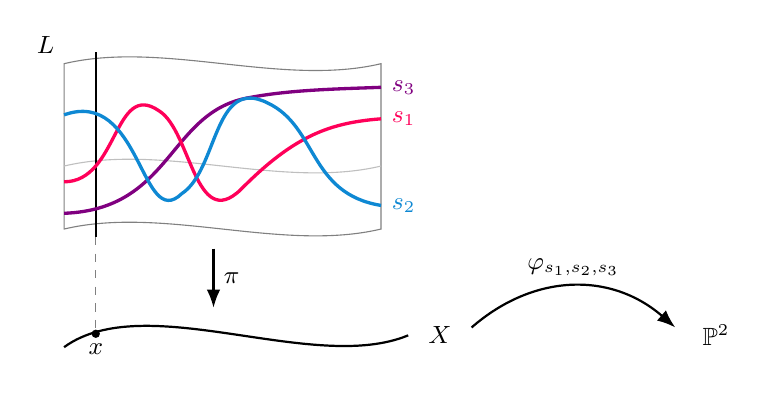
\begin{tikzpicture}[
    x=1.15cm, y=1cm,
    >=Latex,
    section/.style={very thick},
    every node/.style={font=\small}
]
    % A local picture of the line bundle and its zero section.
    \draw[gray] (0,1.35)
        .. controls (1.1,1.65) and (2.4,1.05) .. (3.5,1.35)
        -- (3.5,3.45)
        .. controls (2.4,3.15) and (1.1,3.75) .. (0,3.45)
        -- cycle;
    \node[above left] at (0,3.45) {$L$};
    \draw[gray!50] (0,2.15)
        .. controls (1.1,2.45) and (2.4,1.85) .. (3.5,2.15);

    % The fiber over the marked point x.
    \draw[thick] (0.35,1.25) -- (0.35,3.6);
    \draw[dashed,gray] (0.35,1.25) -- (0.35,0.02);

    % Three sections, labeled at the right edge of the bundle patch.
    \draw[section,violet] (0,1.55)
        .. controls (1.2,1.6) and (1.15,2.85) .. (2.05,3.02)
        .. controls (2.5,3.12) and (3.05,3.13) .. (3.5,3.15)
        node[right] {$s_3$};
    \draw[section,red!65!magenta] (0,1.95)
        .. controls (0.6,1.95) and (0.55,3.25) .. (1.05,2.85)
        .. controls (1.4,2.6) and (1.45,1.3) .. (1.95,1.85)
        .. controls (2.55,2.55) and (2.95,2.7) .. (3.5,2.75)
        node[right] {$s_1$};
    \draw[section,cyan!70!blue] (0,2.8)
        .. controls (0.85,3.15) and (0.85,1.3) .. (1.3,1.8)
        .. controls (1.7,2.1) and (1.65,3.3) .. (2.25,2.95)
        .. controls (2.8,2.65) and (2.7,1.8) .. (3.5,1.65)
        node[right] {$s_2$};

    % Projection to the base and the induced projective map.
    \draw[thick] (0,-0.15)
        .. controls (0.9,0.6) and (2.75,-0.5) .. (3.8,0);
    \fill (0.35,0.02) circle (1.5pt) node[below] {$x$};
    \draw[->,thick] (1.65,1.1) -- (1.65,0.35)
        node[midway,right] {$\pi$};
    \node at (4.15,0) {$X$};
    \draw[->,thick] (4.5,0.1)
        .. controls (5.2,0.8) and (6.05,0.8) .. (6.75,0.1)
        node[midway,above] {$\vf_{s_1,s_2,s_3}$};
    \node at (7.2,0) {$\bP^2$};
\end{tikzpicture}
\end{center}

From here we have a map
\[
\vf_{s_1,s_2,s_3}:X\to \bP^2,\quad x\mapsto [s_1(x):s_2(x):s_3(x)].
\]
This is an abuse of notation because \(s_i(x)\) is a vector, not a number. But it suffices to pick an isomorphism. This map is well defined when \(X\) is such that not all the sections we've chosen vanish at \(x\). (This is basepoint freeness).

If we only want a map depending only on \(L\), then we can 
\begin{enumerate}
    \item pick a basis \(s_0,\dots,s_r\) for \(H^0(X,L)\) (space of regular sections of \(L\) and let \(\vf_L:= \vf_{s_0,\dots,s_r}\).
    \item \(\vf_L: X\to \bP(H^0(X,L)^\vee)\) with \(x\mapsto [``\ev_X:H^0(X,L)\to k,\ s\mapsto s(x)'']\). This is highly undefined! So we should be screaming.
\end{enumerate}

\begin{Def}
    A line bundle \(L\) is basepoint free if for every
    \(x\in X\), there exists \(s\in H^0(X,L)\)
    such that \(s(x)\neq 0\).

    If \(H^0(X,L)\) is finite dimensional, this implies
    that any basis \(s_0,\dots,s_r\) has no common zero.
    Hence it defines a morphism
    \[
        \vf_L:X\to\bP^r,\qquad
        x\mapsto[s_0(x):\cdots:s_r(x)].
    \]
\end{Def}

\begin{Ex}
(...) We have a map \(\bP^2\to\bP^2\) which restricted to the torus is the identity \((s,t,1)\mapsto (s,t,1)\).
\begin{center}
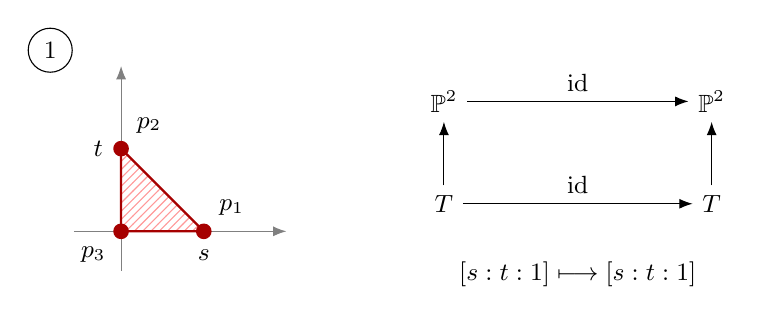
\begin{tikzpicture}[
    x=1cm, y=1cm, >=Latex,
    every node/.style={font=\small},
    lattice point/.style={circle,fill=red!65!black,inner sep=2pt}
]
    \node[draw,circle,inner sep=3pt] at (-0.9,2.3) {$1$};
    \draw[->,gray] (-0.6,0) -- (2.1,0);
    \draw[->,gray] (0,-0.5) -- (0,2.1);
    \path[pattern=north east lines,pattern color=red!40]
        (0,0) -- (1.05,0) -- (0,1.05) -- cycle;
    \draw[thick,red!65!black]
        (0,0) -- (1.05,0) -- (0,1.05) -- cycle;
    \node[lattice point,label=below left:{$p_3$}] at (0,0) {};
    \node[lattice point,label=above right:{$p_1$},label=below:{$s$}]
        at (1.05,0) {};
    \node[lattice point,label=above right:{$p_2$},label=left:{$t$}]
        at (0,1.05) {};

    \node (source) at (4.1,1.65) {$\bP^2$};
    \node (target) at (7.5,1.65) {$\bP^2$};
    \node (source torus) at (4.1,0.35) {$T$};
    \node (target torus) at (7.5,0.35) {$T$};
    \draw[->] (source) -- (target) node[midway,above] {$\mathrm{id}$};
    \draw[->] (source torus) -- (target torus)
        node[midway,above] {$\mathrm{id}$};
    \draw[->] (source torus) -- (source);
    \draw[->] (target torus) -- (target);
    \node at (5.8,-0.55) {$[s:t:1]\longmapsto[s:t:1]$};
\end{tikzpicture}
\end{center}
\end{Ex}

\begin{Ex}
We could remain in \(\bP^2\) and scale the triangle by 2!
\begin{center}
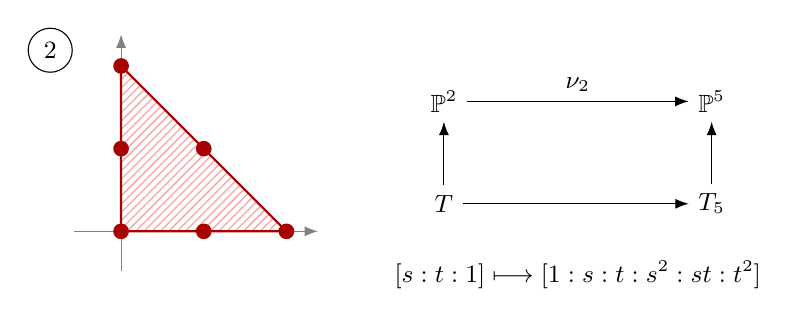
\begin{tikzpicture}[
    x=1cm, y=1cm, >=Latex,
    every node/.style={font=\small},
    lattice point/.style={circle,fill=red!65!black,inner sep=2pt}
]
    \node[draw,circle,inner sep=3pt] at (-0.9,2.3) {$2$};
    \draw[->,gray] (-0.6,0) -- (2.5,0);
    \draw[->,gray] (0,-0.5) -- (0,2.5);
    \path[pattern=north east lines,pattern color=red!40]
        (0,0) -- (2.1,0) -- (0,2.1) -- cycle;
    \draw[thick,red!65!black]
        (0,0) -- (2.1,0) -- (0,2.1) -- cycle;
    \foreach \point in {(0,0),(1.05,0),(2.1,0),(0,1.05),(1.05,1.05),(0,2.1)}
        \node[lattice point] at \point {};

    \node (source) at (4.1,1.65) {$\bP^2$};
    \node (target) at (7.5,1.65) {$\bP^5$};
    \node (source torus) at (4.1,0.35) {$T$};
    \node (target torus) at (7.5,0.35) {$T_5$};
    \draw[->] (source) -- (target) node[midway,above] {$\nu_2$};
    \draw[->] (source torus) -- (target torus);
    \draw[->] (source torus) -- (source);
    \draw[->] (target torus) -- (target);
    \node at (5.8,-0.55)
        {$[s:t:1]\longmapsto[1:s:t:s^2:st:t^2]$};
\end{tikzpicture}
\end{center}
Here \(T_5\) denotes the dense torus of \(\bP^5\).
This is the polytope of the divisor \(2D\), where \(D=\{z=0\}\). We get the map
\[
\nu_2:\bP^2\to\bP^5,\quad T\to T_5,\quad [s:t:1]\mapsto [1:s:t:s^2:st:t^2].
\]
If we think of \((s,t,1)\cdot(x,y,z)=(sx,ty,z)\) then the map at the level of projective spaces is 
\[
[x:y:z]\mapsto[z^2:zx:zy:x^2:xy:y^2].
\]
Here \(\vf(\bP^2)\) is the Veronese surface in \(\bP^5\).
\end{Ex}

\Needspace{13cm}
\begin{Ex}
    Consider now this polytope. 
    \begin{center}
    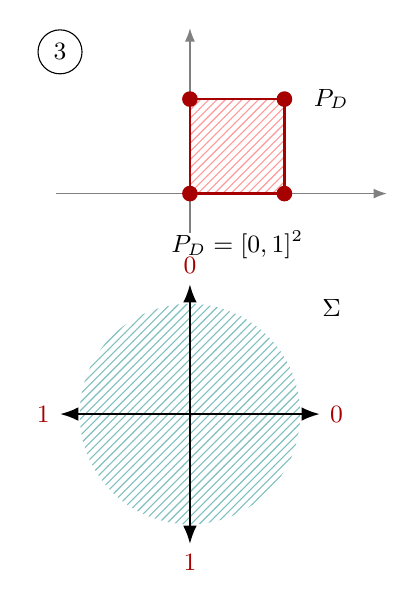
\begin{tikzpicture}[
        x=1cm, y=1cm, >=Latex,
        every node/.style={font=\small},
        lattice point/.style={circle,fill=red!65!black,inner sep=2pt}
    ]
        \node[draw,circle,inner sep=3pt] at (-1.65,4.6) {$3$};

        % The polytope P_D in the character lattice.
        \begin{scope}[yshift=2.8cm]
            \draw[->,gray] (-1.7,0) -- (2.5,0);
            \draw[->,gray] (0,-0.5) -- (0,2.1);
            \path[pattern=north east lines,pattern color=red!40]
                (0,0) rectangle (1.2,1.2);
            \draw[thick,red!65!black] (0,0) rectangle (1.2,1.2);
            \foreach \point in {(0,0),(1.2,0),(1.2,1.2),(0,1.2)}
                \node[lattice point] at \point {};
            \node[right] at (1.45,1.2) {$P_D$};
            \node at (0.6,-0.65) {$P_D=[0,1]^2$};
        \end{scope}

        % The four maximal cones of the fan, with divisor coefficients.
        \foreach \angle in {0,90,180,270} {
            \path[pattern=north east lines,pattern color=teal!50]
                (0,0) -- (\angle:1.4)
                arc[start angle=\angle,delta angle=90,radius=1.4]
                -- cycle;
        }
        \draw[->,thick] (0,0) -- (1.65,0)
            node[right,text=red!65!black] {$0$};
        \draw[->,thick] (0,0) -- (0,1.65)
            node[above,text=red!65!black] {$0$};
        \draw[->,thick] (0,0) -- (-1.65,0)
            node[left,text=red!65!black] {$1$};
        \draw[->,thick] (0,0) -- (0,-1.65)
            node[below,text=red!65!black] {$1$};
        \node at (1.8,1.35) {$\Sg$};
    \end{tikzpicture}
    \end{center}
    \begin{itemize}
        \item From the right ray we get \(x\geq 0\),
        \item The top ray, \(y\geq 0\).
        \item Left gives \(-x\geq -1\) or \(x\leq 1\), and 
        \item Down gives \(-y\geq -1\) or \(y\leq 1\).
    \end{itemize}
    This is \(X_\Sg=\bP^1\x\bP^1\). The map is 
    \[
        \begin{aligned}
            \vf:\bP^1\x\bP^1 &\longrightarrow \bP^3,\\
            T_{\bP^1\x\bP^1} &\longrightarrow T_{\bP^3},\\
            ([s:1],[t:1]) &\longmapsto [1:s:t:st].
        \end{aligned}
    \]
    At the level of projective spaces this map is 
    \[
        ((x_1,x_2),(y_1,y_2))\mapsto(x_2y_2,x_1y_2,x_2y_1,x_1y_1).
    \]
\end{Ex}

\Needspace{10cm}
\begin{Ex}
    Let's start breaking things. 
    \begin{center}
    \begin{tikzpicture}[
        x=1cm, y=1cm, >=Latex,
        every node/.style={font=\small},
        lattice point/.style={circle,fill=red!65!black,inner sep=2pt}
    ]
        \node[draw,circle,inner sep=3pt] at (-0.9,2.3) {$4$};
        \draw[->,gray] (-0.6,0) -- (2.1,0);
        \draw[->,gray] (0,-0.5) -- (0,2.1);
        \draw[very thick,red!65!black] (1.05,0) -- (0,1.05);
        \node[lattice point] at (1.05,0) {};
        \node[lattice point] at (0,1.05) {};

        \node (source) at (4.1,1.65) {$\bP^2$};
        \node (target) at (7.5,1.65) {$\bP^1$};
        \node (source torus) at (4.1,0.35) {$T_{\bP^2}$};
        \node (target torus) at (7.5,0.35) {$T_{\bP^1}$};
        \draw[->,dashed] (source) -- (target)
            node[midway,above] {$\vf$};
        \draw[->] (source torus) -- (target torus);
        \draw[->] (source torus) -- (source);
        \draw[->] (target torus) -- (target);
        \node at (5.8,-0.55) {$[s:t:1]\longmapsto[s:t]$};
    \end{tikzpicture}
    \end{center}
    Consider the map
    \[
        \begin{aligned}
            \vf:\bP^2 &\dashrightarrow \bP^1,\\
            T_{\bP^2} &\longrightarrow T_{\bP^1},\qquad
            [s:t:1]\longmapsto[s:t].
        \end{aligned}
    \]
    This corresponds to \([X:Y:Z]\mapsto [X:Y]\) which is not defined at \([0:0:1]\). This is a \emph{rational} map, not regular. In classical geometry, this is projection from \(p=[0:0:1]\) onto the line \(Z=0\). Every other point \(P\) determines the unique line \(pP\), which meets \(Z=0\) at its image. This works everywhere except at \(p\).
    \Needspace{4cm}
    \begin{center}
    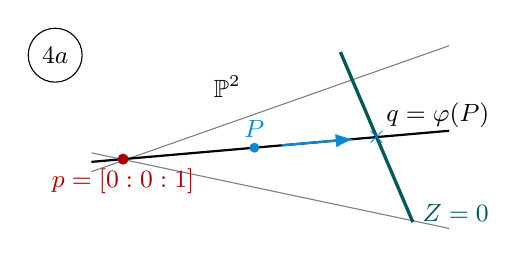
\begin{tikzpicture}[
        x=1.15cm, y=0.8cm, >=Latex,
        every node/.style={font=\small}
    ]
        \node[draw,circle,inner sep=3pt] at (-0.75,1.65) {$4a$};
        % A schematic projective plane and the target line.
        \draw[gray] (-0.35,-0.2) -- (3.6,1.8);
        \draw[gray] (-0.35,0.1) -- (3.6,-1.1);
        \draw[very thick,teal!70!black] (2.4,1.7) -- (3.2,-1);
        \node[right,text=teal!70!black] at (3.2,-0.85) {$Z=0$};
        \node at (1.15,1.15) {$\bP^2$};

        % The line pP meets Z=0 at q.
        \draw[thick] (-0.35,-0.04375) -- (3.6,0.45);
        \fill[red!65!black] (0,0) circle (2pt)
            node[below] {$p=[0:0:1]$};
        \fill[cyan!70!blue] (1.45,0.18125) circle (1.8pt)
            node[above] {$P$};
        \node[text=cyan!70!blue] at (2.8,0.35) {$\times$};
        \node[above right] at (2.8,0.35) {$q=\vf(P)$};
        \draw[->,cyan!70!blue,thick] (1.75,0.21875) -- (2.55,0.31875);
    \end{tikzpicture}
    \end{center}
    One could complain and say diagram 4 doesn't come from a divisor, but instead we say \emph{picky picky} and consider diagram 4b.
    \Needspace{7cm}
    \begin{center}
    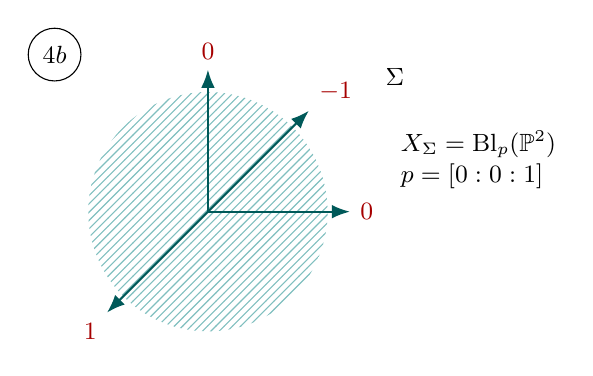
\begin{tikzpicture}[
        x=0.95cm, y=0.95cm, >=Latex,
        every node/.style={font=\small}
    ]
        \node[draw,circle,inner sep=3pt] at (-2.05,2.1) {$4b$};
        % The fan of P^2, subdivided by the exceptional ray (1,1).
        \foreach \start/\sweep in {0/45,45/45,90/135,225/135} {
            \path[pattern=north east lines,pattern color=teal!50]
                (0,0) -- (\start:1.6)
                arc[start angle=\start,delta angle=\sweep,radius=1.6]
                -- cycle;
        }
        \draw[->,thick,teal!70!black] (0,0) -- (1.9,0)
            node[right,text=red!65!black] {$0$};
        \draw[->,thick,teal!70!black] (0,0) -- (0,1.9)
            node[above,text=red!65!black] {$0$};
        \draw[->,thick,teal!70!black] (0,0) -- (1.35,1.35)
            node[above right,text=red!65!black] {$-1$};
        \draw[->,thick,teal!70!black] (0,0) -- (-1.35,-1.35)
            node[below left,text=red!65!black] {$1$};
        \node at (2.5,1.8) {$\Sg$};
        \node[right,align=left] at (2.45,0.7)
            {$X_\Sg=\Bl_p(\bP^2)$\\$p=[0:0:1]$};
    \end{tikzpicture}
    \end{center}
    This is the blowup of \(\bP^2\) at a point, \(X_\Sg=\Bl_{[0:0:1]}(\bP^2)\). 
    \begin{itemize}
        \item The right ray gives \(x\geq 0\),
        \item the \((1,1)\) ray gives \(x+y\geq 1\).
        \item The top one gives \(y\geq 0\) and
        \item \((-1,-1)\) gives \(x+y\leq 1\).
    \end{itemize}
    \Needspace{4cm}
    And so here we get the same kind of polytope. The maps are 
    \[
    \begin{tikzcd}[column sep=large,row sep=large]
        \Bl_{[0:0:1]}(\bP^2)
            \arrow[d,"\pi"'] \arrow[dr,"\vf_D"] & \\
        \bP^2 \arrow[r,dashed,"\vf"'] & \bP^1
    \end{tikzcd}
    \]
    \[
        [X:Y:Z]\longmapsto[X:Y].
    \]
    The lift \(\vf_D\) is a regular morphism, but it is not injective.
    \Needspace{9cm}
    \begin{center}
    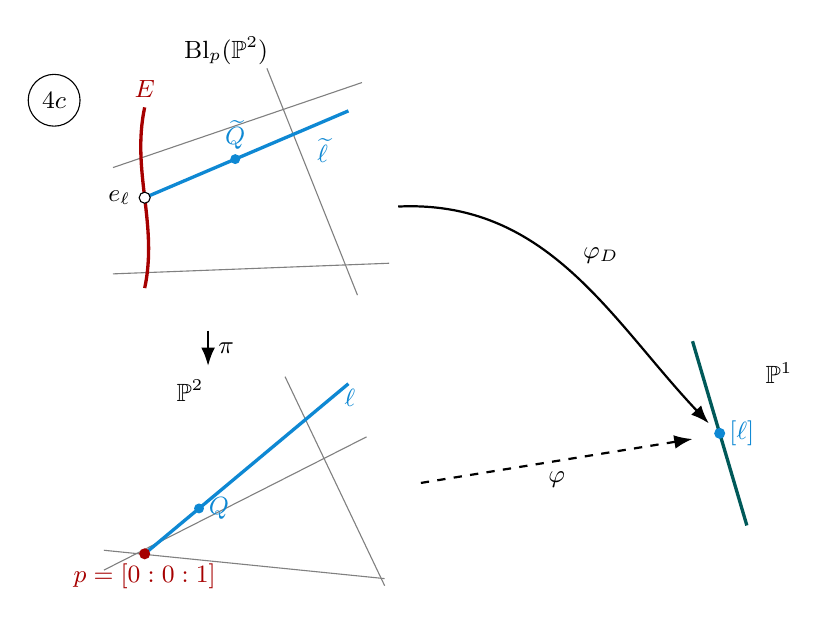
\begin{tikzpicture}[
        x=1.15cm, y=0.9cm, >=Latex,
        every node/.style={font=\small}
    ]
        \node[draw,circle,inner sep=3pt] at (-0.65,6.6) {$4c$};

        % The blown-up plane: a line through p lifts to a curve meeting E.
        \begin{scope}[yshift=3.6cm]
            \node at (1.25,3.3) {$\Bl_p(\bP^2)$};
            \draw[gray] (0,1.65) -- (2.75,2.85);
            \draw[gray] (0,0.15) -- (3.05,0.3);
            \draw[gray] (1.7,3.05) -- (2.7,-0.15);
            \draw[very thick,red!65!black] (0.35,-0.05)
                .. controls (0.5,0.85) and (0.2,1.6) .. (0.35,2.5);
            \node[above,text=red!65!black] at (0.35,2.5) {$E$};
            \draw[very thick,cyan!70!blue] (0.35,1.225) -- (2.6,2.45);
            \node[below right,text=cyan!70!blue] at (2.15,2.205)
                {$\widetilde{\ell}$};
            \filldraw[fill=white,draw=black] (0.35,1.225) circle (2pt);
            \node[left] at (0.3,1.225) {$e_\ell$};
            \fill[cyan!70!blue] (1.35,1.7694) circle (1.8pt)
                node[above] {$\widetilde{Q}$};
        \end{scope}

        % The original plane, with the blue line ell passing through p.
        \node at (0.85,2.5) {$\bP^2$};
        \draw[gray] (-0.1,-0.03) -- (2.8,1.85);
        \draw[gray] (-0.1,0.25) -- (3,-0.15);
        \draw[gray] (1.9,2.7) -- (3,-0.25);
        \draw[very thick,cyan!70!blue] (0.35,0.2) -- (2.6,2.6);
        \node[right,text=cyan!70!blue] at (2.45,2.4) {$\ell$};
        \fill[red!65!black] (0.35,0.2) circle (2pt)
            node[below] {$p=[0:0:1]$};
        \fill[cyan!70!blue] (0.95,0.84) circle (1.8pt)
            node[right] {$Q$};
        \draw[->,thick] (1.05,3.35) -- (1.05,2.85)
            node[midway,right] {$\pi$};

        % Both blue curves determine the same point of the target P^1.
        \draw[very thick,teal!70!black] (6.4,3.2) -- (7,0.6);
        \node[right] at (7.1,2.75) {$\bP^1$};
        \fill[cyan!70!blue] (6.7,1.9) circle (2pt)
            node[right] {$[\ell]$};
        \draw[->,thick] (3.15,5.1)
            .. controls (4.8,5.2) and (5.5,3.5) .. (6.58,2.04)
            node[midway,above right] {$\vf_D$};
        \draw[->,dashed,thick] (3.4,1.2) -- (6.4,1.82)
            node[midway,below] {$\vf$};
    \end{tikzpicture}
    \end{center}
    Away from the exceptional divisor \(E=\pi^{-1}(p)\), the lift
    agrees with the projection \([X:Y:Z]\mapsto[X:Y]\).
    A point \(e_\ell\in E\cong\bP^1\) records a tangent direction at
    \(p\), equivalently a line \(\ell\) through \(p\). The map
    \(\vf_D\) sends it to the corresponding point \([\ell]\) of the
    target, so \(\vf_D|_E:E\to\bP^1\) is an isomorphism.
    The blowup map \(\pi\) contracts all of \(E\) to \(p\).
    The map \(\vf_D\) is not injective because each fiber is the strict
    transform \(\widetilde{\ell}\) of a line through \(p\), a copy of
    \(\bP^1\).
\end{Ex}

\Needspace{13cm}
\begin{Ex}
    Keep the blowup fan and assign coefficient \(1\) to \((-1,-1)\)
    and \(0\) to the other rays. The polytope is the standard triangle.
    \begin{center}
    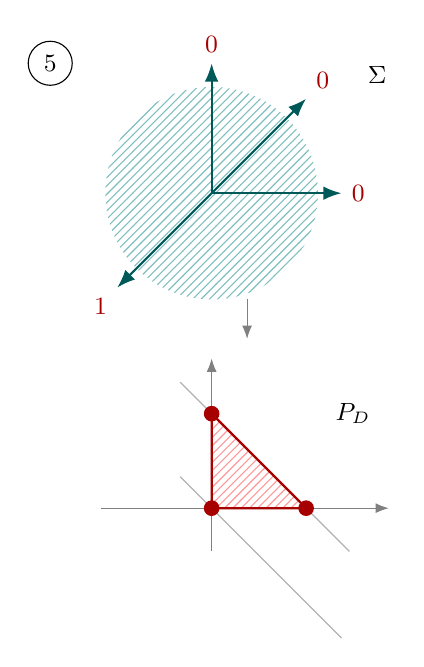
\begin{tikzpicture}[
        x=1cm, y=1cm, >=Latex,
        every node/.style={font=\small},
        lattice point/.style={circle,fill=red!65!black,inner sep=2pt}
    ]
        \node[draw,circle,inner sep=3pt] at (-2.05,5.65) {$5$};

        % The blowup fan, now with coefficient zero on the exceptional ray.
        \begin{scope}[yshift=4cm]
            \foreach \start/\sweep in {0/45,45/45,90/135,225/135} {
                \path[pattern=north east lines,pattern color=teal!50]
                    (0,0) -- (\start:1.35)
                    arc[start angle=\start,delta angle=\sweep,radius=1.35]
                    -- cycle;
            }
            \draw[->,thick,teal!70!black] (0,0) -- (1.65,0)
                node[right,text=red!65!black] {$0$};
            \draw[->,thick,teal!70!black] (0,0) -- (0,1.65)
                node[above,text=red!65!black] {$0$};
            \draw[->,thick,teal!70!black] (0,0) -- (1.2,1.2)
                node[above right,text=red!65!black] {$0$};
            \draw[->,thick,teal!70!black] (0,0) -- (-1.2,-1.2)
                node[below left,text=red!65!black] {$1$};
            \node at (2.1,1.5) {$\Sg$};
        \end{scope}
        \draw[->,gray] (0.45,2.65) -- (0.45,2.15);

        % The extra inequality x+y >= 0 is redundant for this triangle.
        \draw[->,gray] (-1.4,0) -- (2.25,0);
        \draw[->,gray] (0,-0.55) -- (0,1.9);
        \draw[gray!60] (-0.4,0.4) -- (1.65,-1.65);
        \draw[gray!60] (-0.4,1.6) -- (1.75,-0.55);
        \path[pattern=north east lines,pattern color=red!40]
            (0,0) -- (1.2,0) -- (0,1.2) -- cycle;
        \draw[thick,red!65!black]
            (0,0) -- (1.2,0) -- (0,1.2) -- cycle;
        \foreach \point in {(0,0),(1.2,0),(0,1.2)}
            \node[lattice point] at \point {};
        \node[right] at (1.45,1.2) {$P_D$};
    \end{tikzpicture}
    \end{center}
    The divisor is the pullback of a hyperplane, and the associated map
    is the blowdown
    \[
        \Bl_{[0:0:1]}(\bP^2)\xrightarrow{\pi}\bP^2.
    \]
    This is a regular birational morphism: it restricts to an
    isomorphism away from \(E\) and \(p=[0:0:1]\). It is not an
    isomorphism because it contracts the entire exceptional curve
    \(E\cong\bP^1\) to \(p\).
    This divisor is basepoint free but not ample, since the maps
    associated to all positive multiples still contract \(E\).
\end{Ex}

\Needspace{6cm}
We can summarize the relation between divisors and their associated
maps as follows. Let \(D\) be a Cartier divisor on a projective variety
\(X\), and use the complete linear system \(|D|\).
\begin{itemize}
    \item \textbf{Rational map.} When \(|D|\) is nonempty, it determines
    a rational map \(\vf_D\). Its section formula is defined wherever
    the global sections of \(\cO_X(D)\) do not all vanish.
    \item \textbf{Basepoint free.} The divisor \(D\) is basepoint free
    if this section formula is defined at every point. It then gives
    a regular morphism on all of \(X\).
    \item \textbf{Ample.} The divisor \(D\) is ample if some positive
    multiple \(mD\) is very ample, equivalently if \(\vf_{mD}\) is a
    closed embedding for some integer \(m>0\).
    \item \textbf{Very ample.} The divisor \(D\) is very ample if
    \(\vf_D\) itself is a closed embedding, identifying \(X\) with
    its closed image in projective space.
\end{itemize}
\end{document}
